% Created by tikzDevice version 0.12.6 on 2024-05-31 23:46:11
% !TEX encoding = UTF-8 Unicode
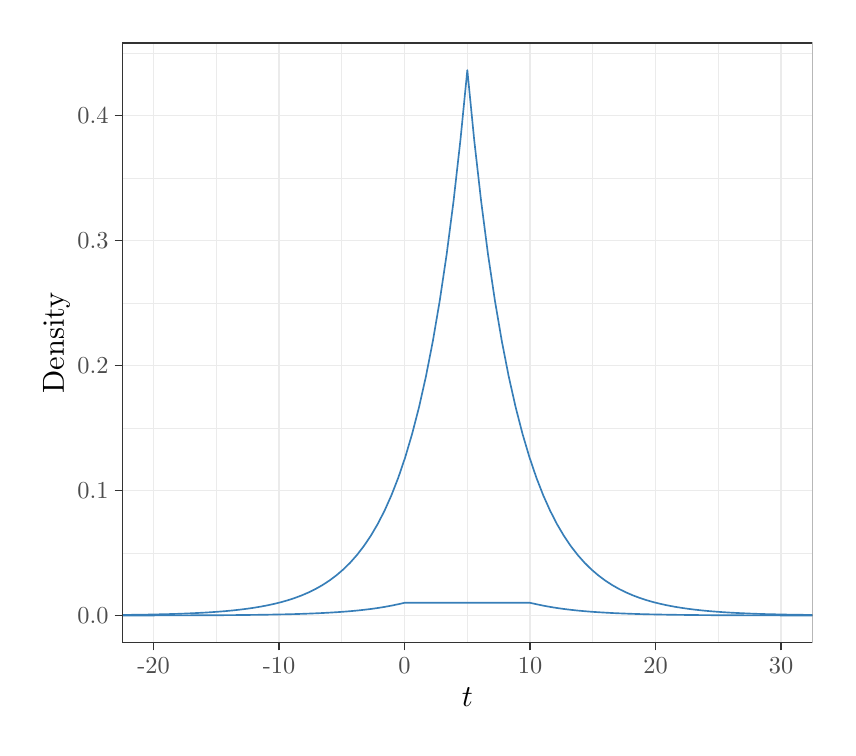
\begin{tikzpicture}[x=1pt,y=1pt]
\definecolor{fillColor}{RGB}{255,255,255}
\path[use as bounding box,fill=fillColor,fill opacity=0.00] (0,0) rectangle (289.08,252.94);
\begin{scope}
\path[clip] (  0.00,  0.00) rectangle (289.08,252.94);
\definecolor{drawColor}{RGB}{255,255,255}
\definecolor{fillColor}{RGB}{255,255,255}

\path[draw=drawColor,line width= 0.6pt,line join=round,line cap=round,fill=fillColor] (  0.00,  0.00) rectangle (289.08,252.94);
\end{scope}
\begin{scope}
\path[clip] ( 34.16, 30.69) rectangle (283.58,247.45);
\definecolor{fillColor}{RGB}{255,255,255}

\path[fill=fillColor] ( 34.16, 30.69) rectangle (283.58,247.45);
\definecolor{drawColor}{gray}{0.92}

\path[draw=drawColor,line width= 0.3pt,line join=round] ( 34.16, 63.11) --
	(283.58, 63.11);

\path[draw=drawColor,line width= 0.3pt,line join=round] ( 34.16,108.28) --
	(283.58,108.28);

\path[draw=drawColor,line width= 0.3pt,line join=round] ( 34.16,153.45) --
	(283.58,153.45);

\path[draw=drawColor,line width= 0.3pt,line join=round] ( 34.16,198.61) --
	(283.58,198.61);

\path[draw=drawColor,line width= 0.3pt,line join=round] ( 34.16,243.78) --
	(283.58,243.78);

\path[draw=drawColor,line width= 0.3pt,line join=round] ( 68.17, 30.69) --
	( 68.17,247.45);

\path[draw=drawColor,line width= 0.3pt,line join=round] (113.52, 30.69) --
	(113.52,247.45);

\path[draw=drawColor,line width= 0.3pt,line join=round] (158.87, 30.69) --
	(158.87,247.45);

\path[draw=drawColor,line width= 0.3pt,line join=round] (204.22, 30.69) --
	(204.22,247.45);

\path[draw=drawColor,line width= 0.3pt,line join=round] (249.57, 30.69) --
	(249.57,247.45);

\path[draw=drawColor,line width= 0.6pt,line join=round] ( 34.16, 40.52) --
	(283.58, 40.52);

\path[draw=drawColor,line width= 0.6pt,line join=round] ( 34.16, 85.69) --
	(283.58, 85.69);

\path[draw=drawColor,line width= 0.6pt,line join=round] ( 34.16,130.86) --
	(283.58,130.86);

\path[draw=drawColor,line width= 0.6pt,line join=round] ( 34.16,176.03) --
	(283.58,176.03);

\path[draw=drawColor,line width= 0.6pt,line join=round] ( 34.16,221.20) --
	(283.58,221.20);

\path[draw=drawColor,line width= 0.6pt,line join=round] ( 45.49, 30.69) --
	( 45.49,247.45);

\path[draw=drawColor,line width= 0.6pt,line join=round] ( 90.84, 30.69) --
	( 90.84,247.45);

\path[draw=drawColor,line width= 0.6pt,line join=round] (136.19, 30.69) --
	(136.19,247.45);

\path[draw=drawColor,line width= 0.6pt,line join=round] (181.54, 30.69) --
	(181.54,247.45);

\path[draw=drawColor,line width= 0.6pt,line join=round] (226.89, 30.69) --
	(226.89,247.45);

\path[draw=drawColor,line width= 0.6pt,line join=round] (272.24, 30.69) --
	(272.24,247.45);
\definecolor{drawColor}{RGB}{55,126,184}

\path[draw=drawColor,line width= 0.6pt,line join=round] ( 34.16, 40.54) --
	( 36.65, 40.54) --
	( 39.14, 40.54) --
	( 41.64, 40.55) --
	( 44.13, 40.55) --
	( 46.63, 40.56) --
	( 49.12, 40.56) --
	( 51.62, 40.57) --
	( 54.11, 40.57) --
	( 56.60, 40.58) --
	( 59.10, 40.59) --
	( 61.59, 40.60) --
	( 64.09, 40.61) --
	( 66.58, 40.62) --
	( 69.08, 40.64) --
	( 71.57, 40.65) --
	( 74.06, 40.67) --
	( 76.56, 40.69) --
	( 79.05, 40.72) --
	( 81.55, 40.75) --
	( 84.04, 40.78) --
	( 86.54, 40.82) --
	( 89.03, 40.87) --
	( 91.52, 40.92) --
	( 94.02, 40.97) --
	( 96.51, 41.04) --
	( 99.01, 41.12) --
	(101.50, 41.21) --
	(103.99, 41.31) --
	(106.49, 41.42) --
	(108.98, 41.56) --
	(111.48, 41.71) --
	(113.97, 41.88) --
	(116.47, 42.08) --
	(118.96, 42.31) --
	(121.45, 42.58) --
	(123.95, 42.88) --
	(126.44, 43.23) --
	(128.94, 43.63) --
	(131.43, 44.09) --
	(133.93, 44.61) --
	(136.42, 45.16) --
	(138.91, 45.16) --
	(141.41, 45.16) --
	(143.90, 45.16) --
	(146.40, 45.16) --
	(148.89, 45.16) --
	(151.39, 45.16) --
	(153.88, 45.16) --
	(156.37, 45.16) --
	(158.87, 45.16) --
	(161.36, 45.16) --
	(163.86, 45.16) --
	(166.35, 45.16) --
	(168.85, 45.16) --
	(171.34, 45.16) --
	(173.83, 45.16) --
	(176.33, 45.16) --
	(178.82, 45.16) --
	(181.32, 45.16) --
	(183.81, 44.61) --
	(186.30, 44.09) --
	(188.80, 43.63) --
	(191.29, 43.23) --
	(193.79, 42.88) --
	(196.28, 42.58) --
	(198.78, 42.31) --
	(201.27, 42.08) --
	(203.76, 41.88) --
	(206.26, 41.71) --
	(208.75, 41.56) --
	(211.25, 41.42) --
	(213.74, 41.31) --
	(216.24, 41.21) --
	(218.73, 41.12) --
	(221.22, 41.04) --
	(223.72, 40.97) --
	(226.21, 40.92) --
	(228.71, 40.87) --
	(231.20, 40.82) --
	(233.70, 40.78) --
	(236.19, 40.75) --
	(238.68, 40.72) --
	(241.18, 40.69) --
	(243.67, 40.67) --
	(246.17, 40.65) --
	(248.66, 40.64) --
	(251.15, 40.62) --
	(253.65, 40.61) --
	(256.14, 40.60) --
	(258.64, 40.59) --
	(261.13, 40.58) --
	(263.63, 40.57) --
	(266.12, 40.57) --
	(268.61, 40.56) --
	(271.11, 40.56) --
	(273.60, 40.55) --
	(276.10, 40.55) --
	(278.59, 40.54) --
	(281.09, 40.54) --
	(283.58, 40.54);

\path[draw=drawColor,line width= 0.6pt,line join=round] ( 34.16, 40.73) --
	( 36.65, 40.76) --
	( 39.14, 40.79) --
	( 41.64, 40.83) --
	( 44.13, 40.87) --
	( 46.63, 40.93) --
	( 49.12, 40.99) --
	( 51.62, 41.05) --
	( 54.11, 41.13) --
	( 56.60, 41.22) --
	( 59.10, 41.33) --
	( 61.59, 41.45) --
	( 64.09, 41.58) --
	( 66.58, 41.74) --
	( 69.08, 41.92) --
	( 71.57, 42.12) --
	( 74.06, 42.36) --
	( 76.56, 42.63) --
	( 79.05, 42.94) --
	( 81.55, 43.30) --
	( 84.04, 43.71) --
	( 86.54, 44.18) --
	( 89.03, 44.72) --
	( 91.52, 45.33) --
	( 94.02, 46.04) --
	( 96.51, 46.86) --
	( 99.01, 47.79) --
	(101.50, 48.86) --
	(103.99, 50.09) --
	(106.49, 51.50) --
	(108.98, 53.12) --
	(111.48, 54.98) --
	(113.97, 57.11) --
	(116.47, 59.55) --
	(118.96, 62.36) --
	(121.45, 65.58) --
	(123.95, 69.27) --
	(126.44, 73.51) --
	(128.94, 78.37) --
	(131.43, 83.95) --
	(133.93, 90.35) --
	(136.42, 97.69) --
	(138.91,106.12) --
	(141.41,115.79) --
	(143.90,126.88) --
	(146.40,139.62) --
	(148.89,154.22) --
	(151.39,170.98) --
	(153.88,190.21) --
	(156.37,212.28) --
	(158.87,237.59) --
	(161.36,212.28) --
	(163.86,190.21) --
	(166.35,170.98) --
	(168.85,154.22) --
	(171.34,139.62) --
	(173.83,126.88) --
	(176.33,115.79) --
	(178.82,106.12) --
	(181.32, 97.69) --
	(183.81, 90.35) --
	(186.30, 83.95) --
	(188.80, 78.37) --
	(191.29, 73.51) --
	(193.79, 69.27) --
	(196.28, 65.58) --
	(198.78, 62.36) --
	(201.27, 59.55) --
	(203.76, 57.11) --
	(206.26, 54.98) --
	(208.75, 53.12) --
	(211.25, 51.50) --
	(213.74, 50.09) --
	(216.24, 48.86) --
	(218.73, 47.79) --
	(221.22, 46.86) --
	(223.72, 46.04) --
	(226.21, 45.33) --
	(228.71, 44.72) --
	(231.20, 44.18) --
	(233.70, 43.71) --
	(236.19, 43.30) --
	(238.68, 42.94) --
	(241.18, 42.63) --
	(243.67, 42.36) --
	(246.17, 42.12) --
	(248.66, 41.92) --
	(251.15, 41.74) --
	(253.65, 41.58) --
	(256.14, 41.45) --
	(258.64, 41.33) --
	(261.13, 41.22) --
	(263.63, 41.13) --
	(266.12, 41.05) --
	(268.61, 40.99) --
	(271.11, 40.93) --
	(273.60, 40.87) --
	(276.10, 40.83) --
	(278.59, 40.79) --
	(281.09, 40.76) --
	(283.58, 40.73);
\definecolor{drawColor}{gray}{0.20}

\path[draw=drawColor,line width= 0.6pt,line join=round,line cap=round] ( 34.16, 30.69) rectangle (283.58,247.45);
\end{scope}
\begin{scope}
\path[clip] (  0.00,  0.00) rectangle (289.08,252.94);
\definecolor{drawColor}{gray}{0.30}

\node[text=drawColor,anchor=base east,inner sep=0pt, outer sep=0pt, scale=  0.88] at ( 29.21, 37.49) {0.0};

\node[text=drawColor,anchor=base east,inner sep=0pt, outer sep=0pt, scale=  0.88] at ( 29.21, 82.66) {0.1};

\node[text=drawColor,anchor=base east,inner sep=0pt, outer sep=0pt, scale=  0.88] at ( 29.21,127.83) {0.2};

\node[text=drawColor,anchor=base east,inner sep=0pt, outer sep=0pt, scale=  0.88] at ( 29.21,173.00) {0.3};

\node[text=drawColor,anchor=base east,inner sep=0pt, outer sep=0pt, scale=  0.88] at ( 29.21,218.17) {0.4};
\end{scope}
\begin{scope}
\path[clip] (  0.00,  0.00) rectangle (289.08,252.94);
\definecolor{drawColor}{gray}{0.20}

\path[draw=drawColor,line width= 0.6pt,line join=round] ( 31.41, 40.52) --
	( 34.16, 40.52);

\path[draw=drawColor,line width= 0.6pt,line join=round] ( 31.41, 85.69) --
	( 34.16, 85.69);

\path[draw=drawColor,line width= 0.6pt,line join=round] ( 31.41,130.86) --
	( 34.16,130.86);

\path[draw=drawColor,line width= 0.6pt,line join=round] ( 31.41,176.03) --
	( 34.16,176.03);

\path[draw=drawColor,line width= 0.6pt,line join=round] ( 31.41,221.20) --
	( 34.16,221.20);
\end{scope}
\begin{scope}
\path[clip] (  0.00,  0.00) rectangle (289.08,252.94);
\definecolor{drawColor}{gray}{0.20}

\path[draw=drawColor,line width= 0.6pt,line join=round] ( 45.49, 27.94) --
	( 45.49, 30.69);

\path[draw=drawColor,line width= 0.6pt,line join=round] ( 90.84, 27.94) --
	( 90.84, 30.69);

\path[draw=drawColor,line width= 0.6pt,line join=round] (136.19, 27.94) --
	(136.19, 30.69);

\path[draw=drawColor,line width= 0.6pt,line join=round] (181.54, 27.94) --
	(181.54, 30.69);

\path[draw=drawColor,line width= 0.6pt,line join=round] (226.89, 27.94) --
	(226.89, 30.69);

\path[draw=drawColor,line width= 0.6pt,line join=round] (272.24, 27.94) --
	(272.24, 30.69);
\end{scope}
\begin{scope}
\path[clip] (  0.00,  0.00) rectangle (289.08,252.94);
\definecolor{drawColor}{gray}{0.30}

\node[text=drawColor,anchor=base,inner sep=0pt, outer sep=0pt, scale=  0.88] at ( 45.49, 19.68) {-20};

\node[text=drawColor,anchor=base,inner sep=0pt, outer sep=0pt, scale=  0.88] at ( 90.84, 19.68) {-10};

\node[text=drawColor,anchor=base,inner sep=0pt, outer sep=0pt, scale=  0.88] at (136.19, 19.68) {0};

\node[text=drawColor,anchor=base,inner sep=0pt, outer sep=0pt, scale=  0.88] at (181.54, 19.68) {10};

\node[text=drawColor,anchor=base,inner sep=0pt, outer sep=0pt, scale=  0.88] at (226.89, 19.68) {20};

\node[text=drawColor,anchor=base,inner sep=0pt, outer sep=0pt, scale=  0.88] at (272.24, 19.68) {30};
\end{scope}
\begin{scope}
\path[clip] (  0.00,  0.00) rectangle (289.08,252.94);
\definecolor{drawColor}{RGB}{0,0,0}

\node[text=drawColor,anchor=base,inner sep=0pt, outer sep=0pt, scale=  1.10] at (158.87,  7.64) {$t$};
\end{scope}
\begin{scope}
\path[clip] (  0.00,  0.00) rectangle (289.08,252.94);
\definecolor{drawColor}{RGB}{0,0,0}

\node[text=drawColor,rotate= 90.00,anchor=base,inner sep=0pt, outer sep=0pt, scale=  1.10] at ( 13.08,139.07) {Density};
\end{scope}
\end{tikzpicture}
